% This is "sig-alternate.tex" V1.9 April 2009
% This file should be compiled with V2.4 of "sig-alternate.cls" April 2009
%
% This example file demonstrates the use of the 'sig-alternate.cls'
% V2.4 LaTeX2e document class file. It is for those submitting
% articles to ACM Conference Proceedings WHO DO NOT WISH TO
% STRICTLY ADHERE TO THE SIGS (PUBS-BOARD-ENDORSED) STYLE.
% The 'sig-alternate.cls' file will produce a similar-looking,
% albeit, 'tighter' paper resulting in, invariably, fewer pages.
%
% ----------------------------------------------------------------------------------------------------------------
% This .tex file (and associated .cls V2.4) produces:
%       1) The Permission Statement
%       2) The Conference (location) Info information
%       3) The Copyright Line with ACM data
%       4) NO page numbers
%
% as against the acm_proc_article-sp.cls file which
% DOES NOT produce 1) thru' 3) above.
%
% Using 'sig-alternate.cls' you have control, however, from within
% the source .tex file, over both the CopyrightYear
% (defaulted to 200X) and the ACM Copyright Data
% (defaulted to X-XXXXX-XX-X/XX/XX).
% e.g.
% \CopyrightYear{2007} will cause 2007 to appear in the copyright line.
% \crdata{0-12345-67-8/90/12} will cause 0-12345-67-8/90/12 to appear in the copyright line.
%
% ---------------------------------------------------------------------------------------------------------------
% This .tex source is an example which *does* use
% the .bib file (from which the .bbl file % is produced).
% REMEMBER HOWEVER: After having produced the .bbl file,
% and prior to final submission, you *NEED* to 'insert'
% your .bbl file into your source .tex file so as to provide
% ONE 'self-contained' source file.
%
% ================= IF YOU HAVE QUESTIONS =======================
% Questions regarding the SIGS styles, SIGS policies and
% procedures, Conferences etc. should be sent to
% Adrienne Griscti (griscti@acm.org)
%
% Technical questions _only_ to
% Gerald Murray (murray@hq.acm.org)
% ===============================================================
%
% For tracking purposes - this is V1.9 - April 2009

\let\mymarginpar\marginpar

\documentclass{sig-alternate}
\usepackage{comment}
\usepackage{amsmath}
\usepackage{amsfonts}
\usepackage{amssymb}
\usepackage{array}
\usepackage{booktabs}
\usepackage{capt-of}
\usepackage{colortbl}
\usepackage{graphicx}
\usepackage{multirow}
\usepackage[center]{subfigure}
\usepackage{pifont}
\usepackage[latin1]{inputenc}
\usepackage{times}
\usepackage{url}
\usepackage{boxedminipage}
\usepackage{xspace}
\usepackage{sepnum}
\usepackage{cite}

% Things to remember
\newenvironment{mynote}%
{\medskip
\noindent
\vspace{2pt}
%\setlength{\fboxsep}{4pt}
%\setlength{\leftmargini}{4pt}
\let\emph=\textbf
\begin{boxedminipage}{.99\columnwidth}\em}%
{\end{boxedminipage}}

\newcommand\remark[1]{%
    \mymarginpar{\raggedright\hbadness=10000\tiny\it #1\par}}
\def\todo#1{\noindent\colorbox{yellow}{X}\remark{{\bf TODO:} #1}}
\def\fixme#1{\noindent\colorbox{yellow}{X}\remark{{\bf FIXME:} #1}}
\def\TODO#1{\todo{#1}}
\def\FIXME#1{\fixme{#1}}

\overfullrule3pt

\begin{document}
%
% --- Author Metadata here ---
\conferenceinfo{WOODSTOCK}{'97 El Paso, Texas USA}
%\CopyrightYear{2007} % Allows default copyright year (200X) to be over-ridden - IF NEED BE.
%\crdata{0-12345-67-8/90/01}  % Allows default copyright data (0-89791-88-6/97/05) to be over-ridden - IF NEED BE.
% --- End of Author Metadata ---

%\title{STC and Build Success in Jazz}
\title{Is NOT Talking About Your Impact on Others Harmful?}
%\title{Communication Patterns}
%\subtitle{[Extended Abstract]
%\titlenote{A full version of this paper is available as
%\textit{Author's Guide to Preparing ACM SIG Proceedings Using
%\LaTeX$2_\epsilon$\ and BibTeX} at
%\texttt{www.acm.org/eaddress.htm}}}

%
% You need the command \numberofauthors to handle the 'placement
% and alignment' of the authors beneath the title.
%
% For aesthetic reasons, we recommend 'three authors at a time'
% i.e. three 'name/affiliation blocks' be placed beneath the title.
%
% NOTE: You are NOT restricted in how many 'rows' of
% "name/affiliations" may appear. We just ask that you restrict
% the number of 'columns' to three.
%
% Because of the available 'opening page real-estate'
% we ask you to refrain from putting more than six authors
% (two rows with three columns) beneath the article title.
% More than six makes the first-page appear very cluttered indeed.
%
% Use the \alignauthor commands to handle the names
% and affiliations for an 'aesthetic maximum' of six authors.
% Add names, affiliations, addresses for
% the seventh etc. author(s) as the argument for the
% \additionalauthors command.
% These 'additional authors' will be output/set for you
% without further effort on your part as the last section in
% the body of your article BEFORE References or any Appendices.

\numberofauthors{2} %  in this sample file, there are a *total*
% of EIGHT authors. SIX appear on the 'first-page' (for formatting
% reasons) and the remaining two appear in the \additionalauthors section.
%
\author{
% You can go ahead and credit any number of authors here,
% e.g. one 'row of three' or two rows (consisting of one row of three
% and a second row of one, two or three).
%
% The command \alignauthor (no curly braces needed) should
% precede each author name, affiliation/snail-mail address and
% e-mail address. Additionally, tag each line of
% affiliation/address with \affaddr, and tag the
% e-mail address with \email.
%
% 1st. author
\alignauthor
Adrian Schr{\"o}ter\\
       \affaddr{Univeristy of Victoria, Canada}\\
       %\affaddr{1932 Wallamaloo Lane}\\
       %\affaddr{Wallamaloo, New Zealand}\\
       \email{schadr@uvic.ca}
% 2nd. author
\alignauthor
Daniela Damian\\
       \affaddr{University of Victoria, Canada}\\
%       \affaddr{P.O. Box 1212}\\
%       \affaddr{Dublin, Ohio 43017-6221}\\
       \email{danielad@cs.uvic.ca}
%% 3rd. author
%\alignauthor Lars Th{\o}rv{\"a}ld\titlenote{This author is the
%one who did all the really hard work.}\\
%       \affaddr{The Th{\o}rv{\"a}ld Group}\\
%       \affaddr{1 Th{\o}rv{\"a}ld Circle}\\
%       \affaddr{Hekla, Iceland}\\
%       \email{larst@affiliation.org}
%\and  % use '\and' if you need 'another row' of author names
%% 4th. author
%\alignauthor Lawrence P. Leipuner\\
%       \affaddr{Brookhaven Laboratories}\\
%       \affaddr{Brookhaven National Lab}\\
%       \affaddr{P.O. Box 5000}\\
%       \email{lleipuner@researchlabs.org}
%% 5th. author
%\alignauthor Sean Fogarty\\
%       \affaddr{NASA Ames Research Center}\\
%       \affaddr{Moffett Field}\\
%       \affaddr{California 94035}\\
%       \email{fogartys@amesres.org}
%% 6th. author
%\alignauthor Charles Palmer\\
%       \affaddr{Palmer Research Laboratories}\\
%       \affaddr{8600 Datapoint Drive}\\
%       \affaddr{San Antonio, Texas 78229}\\
%       \email{cpalmer@prl.com}
}
% There's nothing stopping you putting the seventh, eighth, etc.
% author on the opening page (as the 'third row') but we ask,
% for aesthetic reasons that you place these 'additional authors'
% in the \additional authors block, viz.
%\additionalauthors{Additional authors: John Smith (The Th{\o}rv{\"a}ld Group,
%email: {\texttt{jsmith@affiliation.org}}) and Julius P.~Kumquat
%(The Kumquat Consortium, email: {\texttt{jpkumquat@consortium.net}}).}
%\date{30 July 1999}
% Just remember to make sure that the TOTAL number of authors
% is the number that will appear on the first page PLUS the
% number that will appear in the \additionalauthors section.

\maketitle
\begin{abstract}
Investigating the human aspect of software development is becoming 
prominent in current research. Studies found that the misalignment
between the social and technical dimensions of software work leads to losses in
developer productivity and defects. We study the communication and technical dependencies between developers involved in software integrations and
relate their misalignment to the integration success. Using data from the
IBM Jazz\texttrademark\ project we investigate socio-technical networks in relation to build failure. 
Our findings reveal that the overall socio-technical misalignment  could not distinguish between failed and
successful builds in Jazz\texttrademark,  and that only a small number of
developer pairs that did not communicate about their dependencies were
 related to build failure. The influence of these pairs on the build failure was, however,
very high. We found that if any one of these pairs is present in a
social network of a build, the build had at least an 84\% chance to fail.

%We study the social and technical dependencies between
%developers, because developers are introducing failures into the product they
%develop.

%Observing the social networks constructed from the communication and
%dependencies can reveal harmful patterns that increase the chance of
%introducing errors.


%We build social networks for each software build in the IBM
%Jazz\texttrademark\ project using all discussions and changes related to the
%build.

%I SPOKE ABOUT THESE FINDINGS AT A MORE ABSTRACT LEVEL, ``21'' DOES NOT MEAN
% MUCH UNLESS YOU KNOW THE TOTAL OF PAIRS, ETC. 

%The Jazz\texttrademark\ project contains 21 pairs of developers that are
%technically dependent on each other but did not communicate. If any of the
%aforementioned pairs exists in a build, the build has an 80\% chance of
%failure.
\end{abstract}


\category{D.2.8}{Software Engineering}{Metrics}[complexity measures, \linebreak performance measures]
\category{D.2.9}{Software Engineering}{Management}[Programming Teams]
\category{K.6.1}{Management of Computing and Information Systems}{Project and People Management}[Systems development]
\category{K.6.3}{Management of Computing and Information Systems}{Software Management}[Software development]

\terms{Human Factors, Measurement, Management}

\keywords{Social Networks, Technical Networks, Socio-Technical Networks, Builds, Failures, Socio-Technical Congruence}

\section{Introduction}


Ensuring a smooth progress during software development is key for a project to
stay within budget and on schedule. Failures introduced into the source code
often require an extensive amount of time to fix, especially if caught only at
integration time. Time spent on fixing bugs uses up project budget and
hinders development progress.

In the last decade, research has documented %a growing body of evidence about
multiple reasons for software failures, both on the technical and the human side of
software development. 
On the technical side, studies showed that technical dependencies in the code (e.g.~\cite{zimmermann:icse:2008,gall:icsm:1998}) are powerful predictors of error. 
On the human side, human and organizational factors have been found to strongly affect how
these technical dependencies are handled~\cite{souza:cscw:2004,herbsleb:icse:1999}
 and thus affected %consequently contribute to lower 
 software quality~\cite{cataldo:tse:2009,herbsleb:icis:2006}.
%Communication and 
Coordinating to handle technical dependencies in a project becomes ever more challenging as the level of
interdependencies between tasks increases~\cite{galbraith:book:1973}, especially in large~\cite{curtis:acm:1988} and distributed projects~\cite{damian:icgse:2007,herbsleb:icse:1999}. 
%The alignment between the technical and social dimensions in the project is under
%attack (needs improvement :)).

% Our study of coordination focuses on the interplay between technical and social
% dimensions in teams with high coordination needs and its influence on code
% integrations.
Complementary to studies that relate coordination to software
defects (e.g.~\cite{cataldo:tse:2009}), we investigate
the relationship between team coordination and the success of its code
integration activity. In our previous work~\cite{wolf:icse:2009} we found that
properties of the social networks that represent the communication behavior
% of those wtih technical dependencies in
around software integrations can predict integration failure.
% have a positive relationship to the integration failure.
Here we seek to further our understanding on the influence of communication by
studying the misalignment between technical and social dependencies.

Therefore, we conduct a finer grain investigation at the level of
developer-developer dependency in these work groups. 
Seeking to identify to
what extent the misalignment of technical and social dimensions is linked to coordination failure, we pose the question 
%Hence our
%question 
``\emph{Is NOT talking about your impact on others really
harmful?}''. 
It is important to gain more insights into the communication 
%in a team 
at the level of 
%between 
developers and not the entire team.
Only % since
these insights can be used to more precisely make recommendations that enhance
coordination among team members before the integration fails and thus prevent a project slow down.
%slow down on the project progress.





% Although coordination is mainly measured by investigating communication between developers~\cite{ehrlich:stc:2008,hossain:cscw:2006,hinds:cscw:2006}, it comes with two draw backs.
%Communication is hard to capture completely because developers can use
%communication channels that are hard to record like the infamous water-cooler
%conversation. Furthermore, there may be ways to coordinate without the need to
%communicate, e.g. reviewing the changes other made~\cite{bolici:stc:2009}. Not
%only is communication the most dominant way to coordinate, project teams such
%as the IBM Jazz\texttrademark\ development team, enforce capturing their
%discussions in a central project repository so that anyone anywhere can
%contribute to it.


We study technical dependencies and communication in IBM's Jazz\texttrademark\
project in relation to software builds. Jazz\texttrademark\ is a development
environment that focuses on collaboration support and tightly integrates
programming, communication, and project management (http://www.jazz.net). One
insight from our study is, for example, that out of 16 builds where developers
Adam and Bart changed the same file without communicating about this dependency,
13 builds failed while 3 succeeded, and that this developer pair significantly increased the risk of a
build to fail.

In our methodology we construct socio-technical networks that
represent communication and technical dependencies among developers, and study
them in relation to build outcomes in Jazz. We first seek to validate that
the lack of misalignment between the social and technical dependencies leads to
failure, and then investigate these socio-technical relationships in more
detail at the level of developer-developer dependency. 

Overall, we found that the misalignment between the social and technical
dimensions of work in Jazz did not differentiate between successful and failed
builds. We also identified that only a small number of developer pairs
that did not communicate about their dependencies are statistically related to
build failure. The influence of these pairs on the build failure was, however,
very high. We found that if any one of these pairs is present in a
social network of a build, the build had at least an 84\% chance to fail. 

We
use these findings to discuss the design of collaborative systems that leverage
information about the failure-related developer pairs to determine which
dependencies, if not communicated about, are more critical to the upcoming
build. 




%\newpage%\  \newpage

\section{Research Questions}
Recent research in socio-technical congruence~\cite{cataldo:cscw:2006}, such
as the study of the effects of alignment between social and technical elements
on a development project, found evidence that this alignment influences the
productivity of development teams~\cite{cataldo:cscw:2006}. The idea behind socio-technical congruence (STC) is that if people are technically dependent (e.g. working on interdependent tasks) they should coordinate~\cite{conway:datamination:1968}. If they do not coordinate appropriately, they will slow down progress of others dependent on their tasks. 
%
The slow down occurs when developers need to wait on others' tasks to complete or to make corrections, which in turn, requires more changes~\cite{ehrlich:stc:2008}.

%This is because others are waiting for the task to be completed or needing to
%make corrections due to others' changes, which in turn requires more changes~\cite{ehrlich:stc:2008}.

%I COMMENTED THE TEXT THAT YOU PUT BACK (THIS IS WHERE WE ARE GOING IN CIRCLES
% AND I WANTED TO TALK TO YOU OVER THE PHONE RATHER THAN COMING ACROSS BOSSY
% AND IMPOSING MY VIEW) BECUASE UNLESS WE SAY ``COMPLEMENTARY'' THE SENTENCE
% SIMPLY REPEATS ONE FROM ABOVE. ALSO, IF WE DON'T EXPLAIN IN
% MORE DETAIL WHY COORDINATION AND INTEGRATIONS ARE INTERESTING TO INVESTIGATE,
% THE PAPER IS WEAK OVERALL.  IS THERE ANYTHHING WRONG IN WHAT I SAY BELOW?
%Recent findings show a relation between high socio-technical congruence and
%high productivity. To add to those findings, we study integration failure to
%determine whether STC has a similar relationship to the coordination outcome
%of developers
%  To add to those findings, we ask whether STC has a similar relationship to the
% coordination outcome of developers -- namely, integration failure.  
Complementary to results that imply that high socio-technical congruence is
related to higher productivity, we are asking whether STC has a similar
relationship to an outcome  that is even more tightly related
to developer coordination: integration failure.
If two developers work on interdependent tasks and their changes impact one
another, they should presumably coordinate. Without coordination, they may
introduce failures into the software that make the upcoming integration fail.
Therefore, our first research question:

\begin{enumerate}
\item[RQ1:] Can socio-technical congruence predict integration failure? 
\end{enumerate}

Socio-technical congruence implies the underlying
%is based on the 
concept of socio-technical \emph{gap} between developers. 
When the coordination need of two developers is not met by social interaction, they are said to form a gap.
Research has generally assumed that these gaps are problematic (e.g. \cite{ehrlich:stc:2008}). 
They are responsible for a weak socio-technical congruence and have been said to be responsible for lowering productivity~\cite{cataldo:cscw:2006}. 
Gaps may also be responsible for
developers introducing bugs into the source code, for instance if a develoepr
changes the behavior of a method a co-worker uses, the co-workers code might
break during integration. 
Hence, we investigate if gaps in STC can generally be
related to integration failures.

\begin{enumerate}
\item[RQ2:] Do socio-technical gaps lead to integration failure?  
\end{enumerate}

Having related socio-technical gaps to integration failure, we also seek
explanations as to why they may be failure-related. For example, research suggests that different factors, such as team distribution~\cite{bird:acm:2009} and problem domain~\cite{schroeter:isese:2006}, influence software quality.

The answer to our two research questions and their additional explanation
enable us to devise strategies to fill socio-technical gaps.
These strategies leverage the inter-personal communication that are most
important for the coordination outcome
%
%These strategies 
and are useful for both developers and managers.





%\newpage\ \newpage








\section{Related Work}
Since we are building on the notion of socio-technical congruence we compare technical and social dependencies among developers.
To represent such dependencies among developers a network with the respective
dependency is most appropriate. Thus we first review the research that used
socio-technical networks in software engineering. We also search for patterns
in the project history that concern socio-technical relationships that can be
related to build failure, and thus follow with a review of research in pattern
mining in software engineering. 


\subsection{Networks in Software Engineering}
Three different types of developer networks have been used in software
engineering research: (1) social networks that capture ongoing coordination,
such as communication, (2) technical networks that use source code dependencies to code owners, and (3) socio-technical networks, which
combine social and technical networks. 
%I SUGGEST TAKING THIS SENTENCE OUT BECAUASE YOU DO NOT SAY WHAT TYPE OF
% PATTERNS, AND THE LINK TO THE REVIEW OF PATTERN MINING LITERATURE IS NOW MADE
% AT ONE LEVEL UP. 
%We use those networks to observe
%reoccurring patterns across those networks.

\subsubsection{Social Networks}
Software engineering research is showing an increasing interest in the human side
of software development. To study developer interactions in a software project
several techniques have been borrowed from social sciences. A number of studies
used social network analysis techniques to investigate the relation between
developer social networks and different success measures. These measures range from software quality measures over productivity to
project success.

The mining software repository community described different approaches to mine
social networks from software repositories, like email lists
(e.g.~\cite{bird:msr:2006}). Gonzales-Barahona et al.~\cite{luis:msr:2004} used
social networks to characterize entire projects, in contrast to Yu and
Ramaswamy~\cite{yu:msr:2007} who investigated different roles developers take on
in software projects. The Huang and Liu~\cite{huang:msr:2005} study used a
similar granularity level to draw conclusions about the learning processes in projects.

Wolf et al.~\cite{wolf:ieee:2009} described a methodology for how to mine social
networks from repositories and a study in which they used properties of these
social networks to predict the outcome of integrating the software parts within
teams~\cite{wolf:icse:2009}. Meneely et al.~\cite{meneely:fse:2008} found similar
evidence by extracting developer networks on file level by using code churn
information. Several studies at Microsoft~\cite{bird:acm:2009,nagappan:icse:2008}
showed that different kinds of distance between people that work together on a
binary determine the binaries failure proneness.

Ehrlich et al.~\cite{ehrlich:icgse:2006} investgiated how social networks
can be used to leverage knowledge in distributed teams.
Backstrom et al.~\cite{backstrom:kdd:2006} took a more general approach and investigated the
evolution of large social networks and the information they hold. Chung et
al.~\cite{chung:cpr:07} reported in recent work about behavior of individuals
while performing knowledge intensive tasks. There have been a number of studies
that investigated communication structures to identify good practices
(e.g.~\cite{hinds:cscw:2006,hossain:cscw:2006,bird:fse:2008,xu:hicss:2005,hinds:hicss:2008}).
In contrast to studies of the general development process Marczak studied
social networks to idenify best practices for requirements management
processes~\cite{marczak:re:2008}.

We use social networks to describe the communication and coordination
behavior of developers that contribute to a build.

\subsubsection{Technical Networks}
Much research has been concerned with the technical side of software development.
This technical side is often concerned with the source code. Using code ownership
we can use source code to connect developers constructing a technical network. In
technical networks connections between people are derived from dependencies often
extracted from source code. There are two major ways in which technical networks
have been built: (1) Using explicit source code dependencies and (2) using
implicit source code dependencies.
%\begin{description}
%I REMOVED THE BOLD AND LIST STYLE BECAUSE IT IS NOT AN IMPORTANT CONCEPT IN
% THE OUR PAPER. AND DOES NOT FIT WITH THE
% REST OF THE PAPER. THE TWO TYPES ARE STILL EMPHASIZED, WHICH I THINK IS WHAT
% YOU INTENDED. FEEL FREE TO REVERSE THE STYLE IF YOU THINK THAT THE PREVIOUS
% ONE IS BETTER. 

\emph{Explicit} code dependencies have been used to construct dependency graphs
between source code entities such as classes or methods. These dependency graphs can be constructed either for a complete project or per change made to the source code~\cite{german:ist:2009}.
For instance, Nagappan et al. used several code complexity metrics to build failure prediction models~\cite{nagappan:icse:2006}.

\emph{Implicit} code dependencies are often not visible in the source code
itself. They can be aspects that connect different source code
entities~\cite{tarr:icse:1999}. Source code management systems can make aspects
or other implicit relationships visible by inspecting which files have been
changed together~\cite{nagappan:icse:2005}. 

Zimmermann et
al.~\cite{zimmermann:icse:2008,zimmermann:issre:2007} used technical networks to predict the failure probability of files. Similarly Pinzger et al.~\cite{pinzger:fse:2008} build networks of developers connected via code artifacts to predict failures.
Previous research has also used technical networks for failure prediction by
extraction complexity metrics, such as cyclomatic complexity or object oriented metrics, that are derived from technical networks~\cite{nagappan:icse:2006}.
%I MERGED THE TWO PARAGRAPHS BECAUSE I UNDERSTAND THAT ZIMMERMAN AND PINSGER
% USE THE IMPLICIT DEPENDENCIES. THE ONE SINGLE PARAPRAPH KEEPS THAT ONE IDEA
% IN ONE PLACE, AND THAT IS WHAT I BELIEVE A PARAGRAPH IS MEANT FOR (SOMEHOW
% DIFFERENT FROM YOUR PREFERENCE FOR LENGTH OF PARAGRAPHS). IF THE TWO
% PARAGRAPHS ARE SEPARATE, IT IS UNCLEAR AS TO WHAT ``THOSE TECHNICAL
% NETWORKS'' YOU ARE RERERRING TO. IF YOU MEAN TECHNICAL NETWORKS IN GENERAL
% (WITHOUT INTENDING TO SPECIFY WHETHER IMPLICIT VS. EXPLICIT DEPENDENCIES USED
% IN THEIR CONSTRUCTION) THEN IT MAKES SENSE TO KEEP THE TWO PARAS SEPARATE AND
% REMOVE THE WORD ``THOSE'' IN THE SENTENCE I MENTIONED ABOVE. 
%\end{description}


In our study we construct technical networks for each build in
Jazz\texttrademark\ to describe relations between developers  derived from
co-changed files.
%CAN WE SAY WHETHER THESE ARE EXPLICIT OR IMPLICIT DEPENDENCIES WE ARE USING?
% THE EXPOSITION ABOVE SEEMS OUT OF PLACE OTHERWISE\ldots 

\subsubsection{Socio-Technical Networks}
In recent years research has started to investigate the effect of both social
and technical relations of software developers. Socio-technical networks focus on
developers and connect them with two kinds of edges, social and technical. The
initial idea of investigating the alignment between the communication and
technical dependency between developers was formulated by
Conway~\cite{conway:datamination:1968}.

Expanding on this idea Cataldo et al.~\cite{cataldo:cscw:2006} formulated a coefficient that measures the alignment of the social and technical networks defining the term of socio-technical congruence.
Moreover they observed that higher socio-technical congruence leads to higher developer productivity~\cite{cataldo:cscw:2006}.
Others picked up on that notion and coefficient to further investigate the effect of congruence (e.g.~\cite{valetto:msr:2007}).
Ducheneaut~\cite{ducheneaut:cscw:2005} investigated the evolution of social
and technical relationships of open source project participants to see how those participants become a part of the comunity.

From research on socio-technical congruence emerges the question about what
role socio-technical gaps play. A gap in STC exists if two developers have a
coordination need that is not met by actual coordination behavior. There is a
general tendency to believe that gaps are problematic for projects. Ehrlich et
al.~\cite{ehrlich:stc:2008} investigated gaps and found that files that are changed by developers which form a gap are more prone to change.

To leverage the relation of socio-technical congruence and optimizing task
completion times Sarma et al.~\cite{sarma:icse:2009} developed TESSERACT to
visualize and explore socio technical networks in a project. 

%I SUGGEST WE TAKE THIS SENTENCE OUT BECAUSE WE SHOULD EXPAND A BIT ON THEIR
% STUDIES AND/OR FINDINGS. THIS IS MEANT TO BE RELATED WORK IN SOFTWARE
% ENGINEERING, I BELIEVE. WE THEN CAN REMOVE REF 41. FEEL FREE TO LEAVE IT IN
% IF YOU WISH. 

%Besides software
%engineering research we found studies that look into socio-technical
%relationships in management science (e.g.~\cite{sosa:manage:2004}).

In this work we study ways in which knowledge about socio-technical congruence
can be made actionable \cite{schroeter:rsse:2008}. We study the behavior of
socio-technical networks in teams of developers invovled in a software build
and draw recommendations to prevent build failures.


\subsection{Pattern Mining in Software Engineering}
Patterns in software engineering can be either project specific or more general.
A pattern describes a reoccurring event, such as 
 people updating source code documentation~\cite{schreck:iwpse:2007} after a
 project deadline. The patterns that are found to be beneficial are then used to form templates
 that can be used in the future. Similarly, patterns linked to problems are
 then used to identify harmful events in the future. 
  % I REWORDED THIS TO AVOID THE QUESTION OF WHY DO YOU USE THE WORDS ``GOOD''
 % AND ``BAD'' WITHOUT DEFINING THEM. THEY ARE NOT USED IN THE REMAINING OF THE
 % PAPER SO I THINK THEY CAN BE SAFELY AVOIDED. SEE IF THE TEXT BELOW MAINTAINS
 % THE MEANING YOU INTENDED. 
 %Good patterns are then used to form templates that can be used in the future.
 %Bad patterns on the other hand can be used to identify harmful events that
 %might cause problems. Note that good and bad can be defined in many ways.
 
 %ALSO, MY SUGGESTION IS TO REMVOE THE BOLD AND LIST STYLE. SEE MY SUGGESTION
 % BELOW.
 
%\begin{description}
\emph{Project Specific Patterns}. Schr\"oter et al.~\cite{schroeter:isese:2006}
extracted package usage information and found that using certain packages increases the chance of a file containing a failure. Neuhaus et al.~\cite{neuhaus:ccs:2007} extended on that approach and investigated used packages in relation to vulnerabilities in Mozilla Firefox.
Zimmermann er al.~\cite{zimmermann:oopsla:2005} developed eRose, an Eclipse plug-in that scans a source code repository for co-changed lines and makes recommendations for future changes.

\emph{General Patterns}. Programs such as FindBugs~\cite{cole:oopsla:2006} isolated anti patterns in source code, such as code smells, that have often been observed with failures.
The book ``Design Patterns''~\cite{gamma:1995} gives general guidelines to construct better software by giving examples on working designs.
%\end{description}

In our study we focus on simple patterns that are comprised only of a pair of
developers that are connected via a technical dependency and relate to build
failure.








%\newpage%\ \newpage



%\pagebreak
\section{Methodology}
%I THINK YOU MEANT TO SAY THAT ``THIS SECTION EXPLAINS\ldots'', I DON'T THINK
% THAT ``THE METHODOLOGY \ldots EXPLAINS'' MAKES SENSE. HENCE MY SUGGESTION
% BELOW.

Our methodology to answer our research questions constructs socio-technical
networks in order to analyze coordination behavior in software teams. We use
such networks to analyze socio-technical congruence and socio-technical gaps
both in relation to integration outcome in software projects.
%
%We use data from IBM's Jazz\texttrademark\ repository. 
Below we first describe our methods to collect data on coordination and
integration from the Jazz\texttrademark\ repository. We then describe
the methods we use to construct and analyze social networks associated with these integrations.

\subsection{Data Collection}
In the following we describe what data we use to extract social networks that we extend to socio-technical network.

\subsubsection{Coordination and Integrations in Jazz}
We analyze builds in the Jazz\texttrademark\ repository to study
coordination and integrations in Jazz. 
The Jazz\texttrademark\ team integrates on different levels and in different intervals, for instance on the team or project level in a nightly and weekly interval.
%ONE SENTENCE HERE ABOUT THE TYPE OF INTEGRATIONS THEY HAVE
%(NIGHTLY, WEEKLY, PROJECT-WIDE). 
Each build and therefor integration includes a number of
changesets. A \emph{changeset} consists of changes to one or more files in a
project, comparable to a transaction in the source code management system
Subversion (http://subversion.tigris.org). Furthermore, information about a  build is
stored in the Jazz\texttrademark\ repository. This includes the time the building
process started, if the build succeeded and passed its test cases, and the built
product. But if we refer to the build outcome we are talking about whether it
could be built and if it passed all test cases.

We investigate the Jazz\texttrademark\ builds between April and July 2008.
We choose this time interval because this represents the interval with the most complete history of builds.
The Jazz\texttrademark\ development team deletes builds that are less important due to space reasons.
Thus older builds besides builds that represent important milestones have been deleted.

From this time interval we extracted a total of 244 builds (see
Table~\ref{tab:jazzbuildinfo} for details), specifically 70 failed builds and 174
successful builds. Each build has on average 32 changesets, with a changeset
touching 29 files on average. Note that there are some builds that have only one changeset associated
with them. These are project wide builds that accumulate all changes made by
all teams into one changeset.



\begin{table}[t]
\centering
\begin{tabular}{rrccc}
\toprule
& & Successful & Failed & Total\\
\midrule
&min &1&1&1\\
\#WorkItem & avg  & 16.68&26.52&19.63\\
& max & 111&109&111\\
\midrule
& min & 1&1&1\\
\#ChangeSet & avg  & 26.71&46.27&32.57\\
& max & 227&194&227\\
\midrule
& min & 1&1&1\\
\#Developers & avg  & 19.62&28&22.16\\
& max &64&71&71\\
\bottomrule
\end{tabular}
\caption{Statistics on Jazz data: change sets, work items, 
and developers over successful (227), failed (99) and total builds (328).}
\label{tab:jazzbuildinfo}
\end{table}

\begin{figure}[b]
\centering
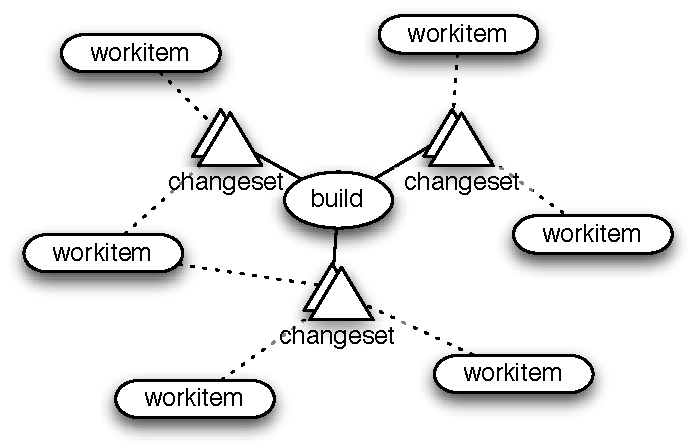
\includegraphics[width=.8\columnwidth]{buildworkitem}
%\vspace{-.3cm}
\caption{Linking workitems to builds using changesets.}
\label{fig:buildtoworkitem}
\end{figure}

\begin{figure}[t]
\centering
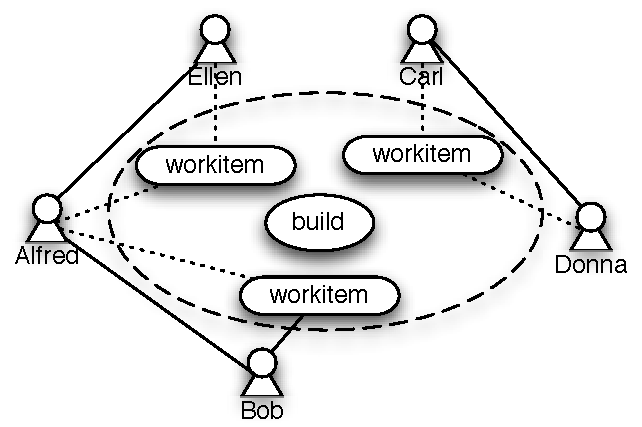
\includegraphics[width=.8\columnwidth]{buildsn}
%\vspace{-.3cm}
\caption{Social network connecting developers through workitem discussions linked to a build}
\label{fig:buildsn}
\end{figure}

\subsubsection{Extracting Social Networks}
We first construct \emph{social networks} to capture the coordination behavior of
developers invovled in a build. We use the information contained in the
Jazz\texttrademark\ workitems for the construction. A \emph{workitem} in Jazz\texttrademark\ is the basic unit of
work. It describes a general task which can be, but is not restricted to, a bug fix or feature request.
Developers coordinate about work on workitems by posting comments in a
discussion board style which we use as conceptualization of their coordination behavior. 

%very much like developers discuss a bug report made in a Bugzilla
%(http://www.bugzilla.org) issue tracker.

We are interested in constructing a social network for each
build in Jazz\texttrademark. 
To create a social network for a given build we proceed in six steps:

\begin{enumerate}
\item Select the build of interest.
\item Extracting changesets that are part of the build.
\item Extracting workitems linked to the retrieved changesets.
\item Extracting developers commenting on a workitem before the build's built time.
%\item Retrieve developers that created the retrieved workitems.
\item Connect all developers commenting on the same workitem.
\end{enumerate}

These steps take us as illustrated in Figure~\ref{fig:buildtoworkitem}
from a build through a changeset to a workitem. From the workitem we are able to
see who contributed to the workitem discussion (see Figure~\ref{fig:buildsn}).
These developers become part of the social network and
share a \emph{social edge} if they made a comment on the same workitem.
% We use the term \emph{social edge} to describe this connection between two
% developer that commented on the same workitem.
Note that all links we use to get from a build to a developer are explicitly contained in
the Jazz\texttrademark\ repository.




\subsubsection{Extending to Socio-Technical Networks}
To construct \emph{socio-technical networks} we use the steps described below
(see Figure~\ref{fig:addtechnicaledge}). We essentially add technical edges to
the build's already constructed social network. In our conceptualization a \emph{technical edge} is a source code
dependency between two developers. A technical dependency between two developers
exists if they changed the same source code file in the build of interest. 

\begin{enumerate}
\item Extract the changesets that are part the build (Figure~\ref{subfig:idcs}).
\item Determine changeset owners and add those  that are not already part
of the social network (Figure~\ref{subfig:adduser}).
\item Add a technical edge between changeset owners that changed the same file (see Figure~\ref{subfig:addedge}).
\end{enumerate}

We thus call a network that contains both social and technical edges a
\emph{socio-technical network}. The developers in the 
socio-technical network that share both a technical and social edge are said to share
a \emph{socio-technical edge}.

%\begin{figure}[t]
%\centering
%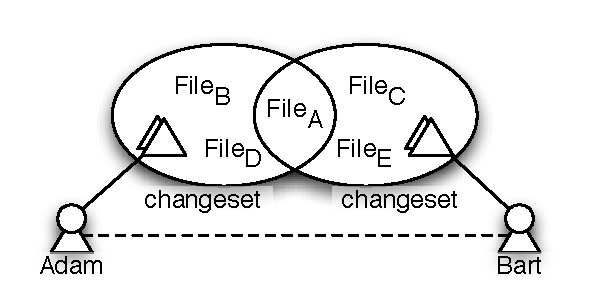
\includegraphics[width=.7\columnwidth]{cochangedfiles}
%%\vspace{-.3cm}
%\caption{Conceptualization of technical relation using co-changed files.}
%\label{fig:technicaldependency}
%\end{figure}

\begin{figure*}[t]
\centering
\subfigure[Identify all changesets related to the social network's build.]{
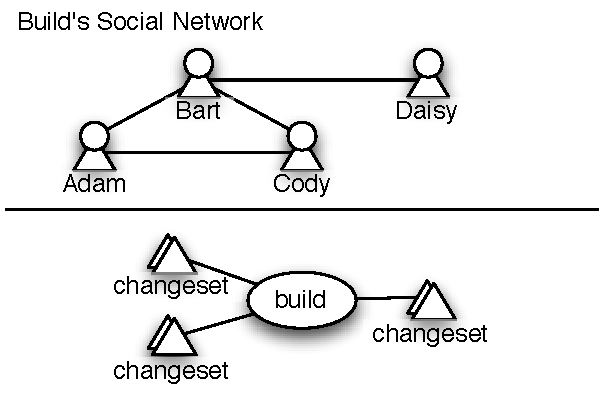
\includegraphics[width=.66\columnwidth]{idcs}
\label{subfig:idcs}
}
\subfigure[Adding changeset owners that are not part of the social network.]{
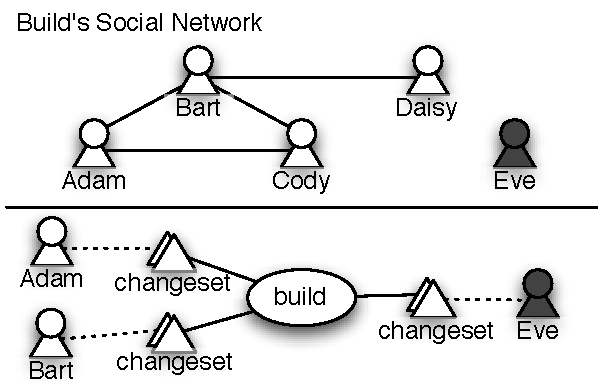
\includegraphics[width=.66\columnwidth]{adduser}
\label{subfig:adduser}
}
\subfigure[Connect Adam and Bart with a technical edge via the co-changed File$_A$.]{
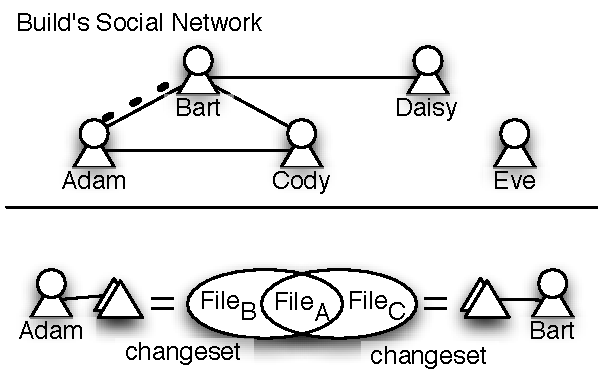
\includegraphics[width=.66\columnwidth]{addedge}
\label{subfig:addedge}
}
%\vspace{-.2cm}
\caption{
Creating a socio-technical network by adding technical dependencies to a build's social-network.}
\label{fig:addtechnicaledge}
\end{figure*}

\subsection{Data Analysis}
We perform two analyses on the networks we constructed,
starting with comparing the socio-technical congruence index of
networks of successful and failed builds, followed by a more detailed
investigation of socio-technical gaps in relation to build outcome.

\subsubsection{Build Outcome and STC Predictive power}
To answer our first research question, we investigate the build outcome and the
socio-technical congruence for all builds. Socio-technical congruence (STC)
describes the match between the coordination needs in a development team as
demanded by technical interdependencies and the ongoing coordination among
developers. 

In calculating the STC index for each build's socio-technical network, we
use the measure defined by Cataldo et al.~\cite{cataldo:cscw:2006}, which is the ratio between the
number of coordination needs that are met and the number of all 
coordination needs.
The index ranges from 0 (no congruencet) to 1 (perfect congruence).

We conceptualize the coordination needs with technical edges and
the ongoing coordination with social edges. Thus the socio-technical congruence
index is determined by the number of socio-technical edges (number of met
coordination needs) over the number of technical-edges (number
of coordination needs). We compute this index for all socio-technical networks.

Since each build has an assigned build outcome (successful
or failed), we split each build's  socio-technical congruence index
into two bins. To determine whether socio-technical congruence can be used to distinguish between
successful and failed builds we perform a Wilcoxon signed rank test.


% \newpage\ \newpage\ \newpage
\subsubsection{Analysis of Socio-Technical Gaps}
Socio-technical gaps occur when coordination needs are not met by ongoing
coordination. As such, we are interested in analyzing pairs of developers that
share a technical edge (implying coordination need) but no social edge (implying
unmet coordination need) in socio-technical networks. We refer to these pairs of
developers as \emph{technical pairs}, and to those that do share a
socio-technical edge (there is no gap) as \emph{socio-technical pairs}. 

To answer our second research question, we are interested in whether the
technical pairs are related to build
failure. Our analysis proceeds in four steps:


%A pair is significant if
%its presence increases the chance of a build being successful or a failure. To
%ensure that making people talk is no harm, we also investigate whether pairs
%developers that share a socio-technical edge are failure related.

%We call a developer pair that only shares a technical edge a \emph{technical
%pair}. We need to mine those technical pairs to identify if they all lead to
%failure (RQ 2). O:

\begin{enumerate}
\item Identify all technical pairs from the socio-technical networks.
\item For each technical pair count occurrences in socio-technical networks of
failed builds.
\item For each technical pair count occurrences in socio-technical networks of
successful builds.
\item Determine if the pair is significantly related to success or failure.
\end{enumerate}

For example, in Table~\ref{tab:contingencytable} we illustrate the analysis of
the technical pair (Adam, Bart). This pair appears in 3 successful builds and in
13 failed builds. Thus it does not appear in 171 successful builds, which is the total number of successful builds minus the number of successful builds the pair appeared in, and it is absent in 57 failed builds.
A Fischer Exact Value test yields significance at a confidence level of $\alpha$ = .05 with a p-value of $4.273\cdot10^{-5}$.

Note that we adjust the p-values of the Fischer Exact Value test to account for multiple hypothesis testing using the Bonferroni adjustment.
The adjustment is necessary because we deal with 961 technical pairs that need to be tested. 

To enable us to discuss the findings as to whether closing socio-technical gaps
are needed to avoid build failure, or which of these gaps are more important to
close, we peform a two additional analyses. 
First we analyze whether the
socio-technical pairs also appear to be build failure-related or not, by
following the same steps as above for socio-technical pairs. 
%
Secondly, we prioritize the developer pairs using the coefficient $p_x$,
which represents the normalizd likelihood of a build
to fail in the presence of the specific pair:

$$p_x\text{=}\frac{ \text{pair}_{failed} / \text{total}_{failed} }
                     { \text{pair}_{failed} / \text{total}_{failed} + \text{pair}_{success} / \text{total}_{successs}}$$ 

The coefficient is comprised of four things: (1) pair$_{failed}$, the number of failed builds where the pair occurred; (2) total$_{failed}$, the number of failed builds; (3) pair$_{success}$, the number of successful builds where the pair occurred; (4) total$_{success}$, the number of successful builds.
This coefficient is normalized with the number of failed and successful builds.
A value closer to one means that the developer pair is strongly related to build
failure. Additionally it describes a probability of failure likelihood that accounts for the imbalance in the data.



%\newpage\ \newpage

\begin{table}[t]
\centering%\vspace{1cm}
\begin{tabular}{rcc}
\toprule
 & successful & failed  \\
 \midrule
(Adam, Bart) & 3 & 13 \\
$\neg$ (Adam, Bart) & 224 & 86\\
\midrule
total&227&99\\\bottomrule
%User3493, User2943 & 3 & 13
\end{tabular}
\caption{Contingency table for technical pair (Adam, Bart) in relation to build
success or failure}
\label{tab:contingencytable}
\end{table}




%\newpage\ \newpage








\section{Results}
In this section we present our findings, starting with the investigation of the relation between socio-technical congruence and build success.
Next we show the results we obtained from analyzing the socio-technical gaps.




\begin{figure}[t]
\centering
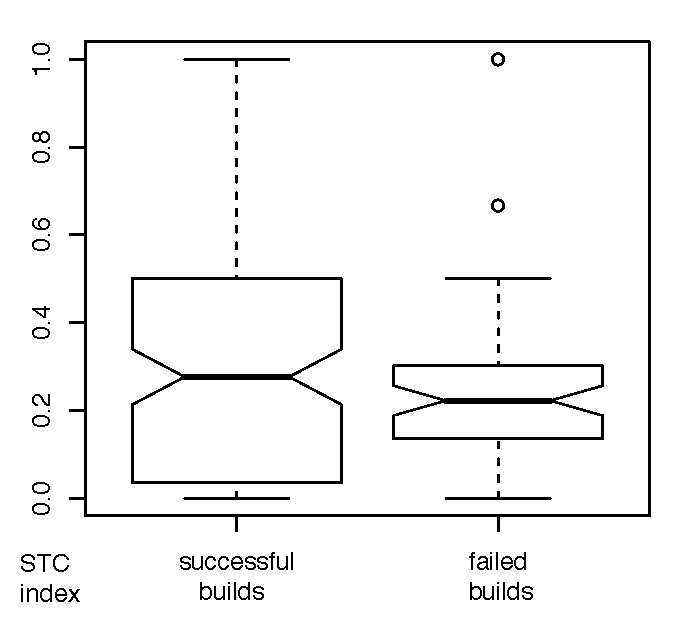
\includegraphics[width=.7\columnwidth]{stcboxplot.pdf}
\vspace{-.3cm}
\caption{Boxplot of the STC index associated with successful (left) and failed
(right) builds.}
\label{fig:stcboxplot}
\end{figure}

\subsection{STC and Build Outcome}
We divide the socio-tecnical networks according to the respective build outcome,
to see whether the socio-technical index~\cite{cataldo:cscw:2006} can be used to determine build success.
After performing a Wilcoxon Signed Rank test with the hypothesis
that the two populations are different at a confidence value of $\alpha$ = .05,
we rejected the hypothesis (p = 0.2135). 
This implies that socio-technical
congruence cannot differentiate between successful and failed builds and thus we
cannot answer our first research question with yes.

The box plot in Figure~\ref{fig:stcboxplot} shows the two distributions of the
networks according to build outcome. 
The medians of both categories (middle line) indicate a STC index of 0.27 and 0.22 for successful and failed builds respectively. 
%The medians are not significantly different, if the notches overlap. 
The upper and lower boundaries of a box
represent the 75\% and 25\% percentile respectively and the wiskers denote the
90\% and 10\% percentiles. All data points outside the 10-90\% interval are shown
as outliers.





\begin{table}[t]
\centering
\begin{tabular}{cccc}
\toprule
Technical Pair & \#successful & \#failed & $p_x$\\
\midrule
Cody-Daisy&  0 & 12 & 1.0000 \\
Adam-Ina & 0 & \phantom{1}8 & 1.0000 \\
Adam-Kim& 0 & \phantom{1}8 & 1.0000 \\
Adam-Nina & 0 & \phantom{1}6 & 1.0000 \\
Fred-Gina& 0 & \phantom{1}6 & 1.0000 \\
Gina-Oliver & 0 & \phantom{1}6 & 1.0000 \\
Adam-Daisy& 1 & 14 & 0.9720\\%67 \\
Bart-Daisy& 1 & \phantom{1}9 & 0.9572\\%127 \\
Adam-Lisa& 1 & \phantom{1}8 & 0.9521\\%204 \\
Bart-Eve & 2 & 11 & 0.9318\\%403 \\
\textbf{Adam}-\textbf{Bart}& \textbf{3} & \textbf{13} & \textbf{0.9150}\\%485 \\
Bart-Cody & 3 & 13 & 0.9150\\%485 \\
Adam-Eve & 4 & 16 & 0.9086\\%162 \\
Daisy-Ina & 3 & 12 & 0.9086\\%162 \\
Cody-Fred& 3 & 10 & 0.8923\\%077 \\
Bart-Herb & 3 & 10 & 0.8923\\%077 \\
Cody-Eve & 5 & 15 & 0.8817\\%568 \\
Adam-Jim & 4 & 11 & 0.8723\\%792 \\
Herb-Paul & 5 & 12 & 0.8564\\%397 \\
Mike-Rob& 6 & 13 & 0.8434\\%004\\
Adam-Fred & 6 & 13 & 0.8434\\%004\\
%
%User11137, User4105 & 0 & 12 & 1.0000 \\
%User2943, User13877 & 0 & 8 & 1.0000 \\
%User7438, User2943 & 0 & 8 & 1.0000 \\
%User2943, User2810 & 0 & 6 & 1.0000 \\
%User8645, User1976 & 0 & 6 & 1.0000 \\
%User8645, User2267 & 0 & 6 & 1.0000 \\
%User11137, User2943 & 1 & 14 & 0.9675\\%908 \\
%User11137, User3493 & 1 & 9 & 0.9504\\%773 \\
%User6012, User2943 & 1 & 8 & 0.9446\\%298 \\
%User3493, User2435 & 2 & 11 & 0.9214\\%387 \\
%User3493, User2943 & 3 & 13 & 0.9023\\%53 \\
%User3493, User4105 & 3 & 13 & 0.9023\\%53 \\
%User2943, User2435 & 4 & 16 & 0.8950\\%695 \\
%User11137, User13877 & 3 & 12 & 0.8950\\%695 \\
%User1976, User4105 & 3 & 10 & 0.8766\\%716 \\
%User3493, User6339 & 3 & 10 & 0.8766\\%716 \\
%User4105, User2435 & 5 & 15 & 0.8648\\%208 \\
%User2943, User9017 & 4 & 11 & 0.8543\\%22 \\
%User6339, User13875 & 5 & 12 & 0.8365\\%498 \\
%User10979, User3385 & 6 & 13 & 0.8220\\%793\\
%User2943, User1976 & 6 & 13 & 0.8220\\%793 \\
\bottomrule
\end{tabular}
\caption{Twenty-one \emph{technical pairs} that are failure-related}
\label{tab:badtechpairs}
\end{table}

\begin{table}[t]
\centering
\begin{tabular}{cccc}
\toprule
Socio-technical Pair & \#successful & \#failed & $p_x$\\
\midrule
Adam-Cody & 0 & \phantom{1}9 & 1.0000 \\
Lisa-Sarah & 0 & \phantom{1}8 & 1.0000 \\
Bart-Ina & 0 & \phantom{1}7 & 1.0000 \\
Tom-Xavier & 0 & \phantom{1}6 & 1.0000 \\
Vince-Xavier & 0 & \phantom{1}6 & 1.0000 \\
Bart-Will & 3 & 13 & 0.9150\\%485 \\
\textbf{Zac}-\textbf{Eve} & \textbf{3} & \textbf{10} & \textbf{0.8923}\\%077 \\
%
%User2943, User4105 & 0 & 9 & 1.0000 \\
%Sarah User3982, User6012 & 0 & 8 & 1.0000 \\
%User3493, User13877 & 0 & 7 & 1.0000 \\
%Tom User1326, Xavier User2267 & 0 & 6 & 1.0000 \\
%Vince User10517, User2267 & 0 & 6 & 1.0000 \\
%User3493, Will User13871 & 3 & 13 & 0.9023\\%53 \\
%Zack User13873, User2435 & 3 & 10 & 0.8766\\%716 \\
\bottomrule
\end{tabular}
\caption{Seven  \emph{socio-technical pairs} that are failure-related}
\label{tab:badstechpairs}
\end{table}


% \subsection{Influence of Technical Dependencies}
\subsection{Socio-technical Gaps and Build Outcome}
We found a total of 961 technical pairs. %. The Fischer Exact Value tests show
While only 21 pairs are significantly correlated with build failure (see
Table~\ref{tab:badtechpairs}), none are correlated with successful builds.
%
Similarly, we investigated whether specific socio-technical pairs influence
build outcome and found that 7 pairs significantly correlated with build
failure (see Table~\ref{tab:badstechpairs}) while none correlated with successful builds.
Note that we use fictitious names for confidentiality reasons.

\begin{figure}[t]
\centering
\vspace{-1cm}
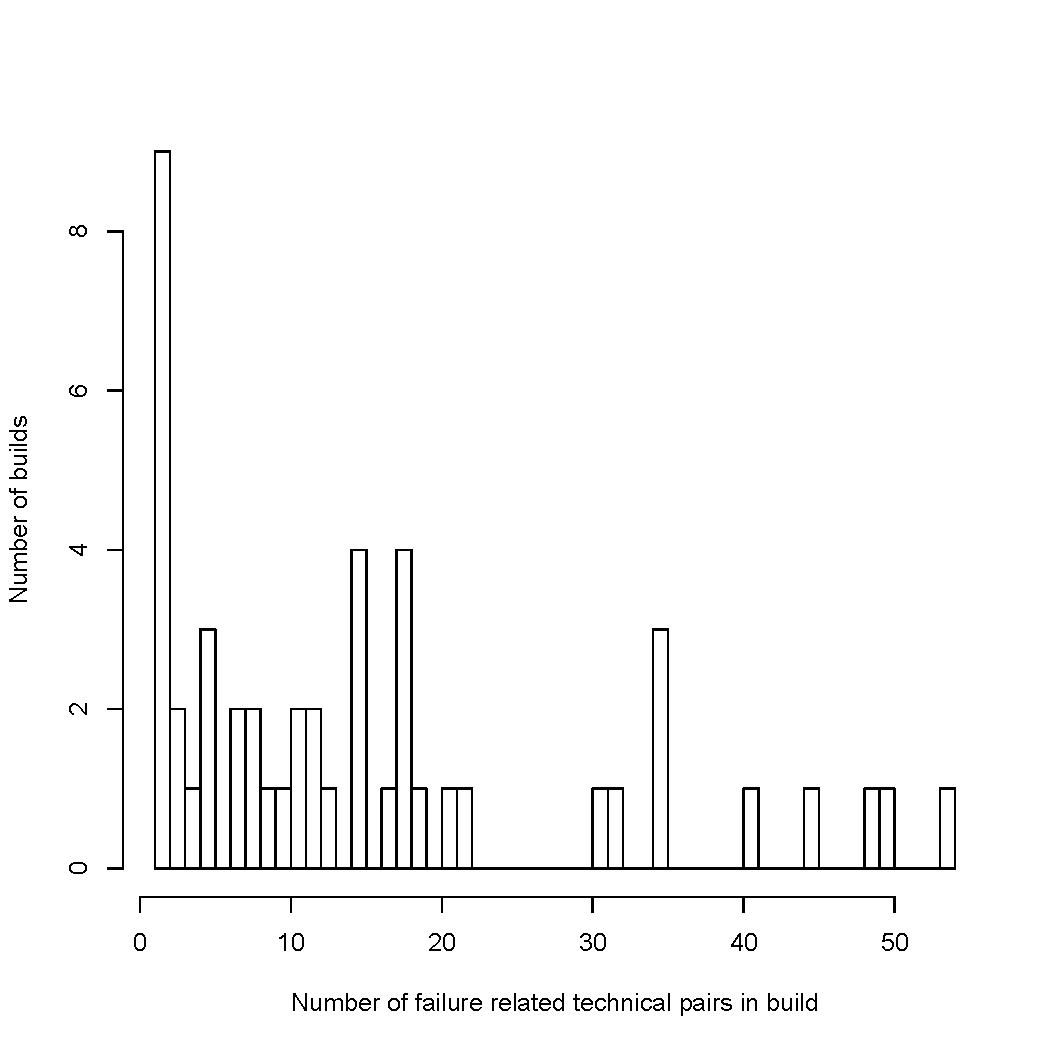
\includegraphics[width=\columnwidth]{builddistribution}
%\vspace{-.75cm}
\caption{Histogram plotting how many builds have a certain number of failure-reated technical pairs.}
\label{fig:builddistribution}
\end{figure}


We rank the the 28 identified technical and socio-technical pairs 
(see Tables~\ref{tab:badtechpairs} and~\ref{tab:badstechpairs}) by the coefficient $p_{x}$.
This coefficient indicates the strength of relationship between the developer pair and build failure. 
In other words $p_{x}$ represents the normalized likelihood that a build that has the
respective pair will fail. Note that all $p_{x}$ values are above 84\%. 
Below we describe how to read Tables~\ref{tab:badtechpairs}
and~\ref{tab:badstechpairs}:

\begin{description}
\item[Technical Pairs.] Table~\ref{tab:badtechpairs} lists all 21 technical pairs that are significant
according to the Fischer Exact Value test and ranks them according to the
coefficient $p_x$. For instance, the developer pair (Adam, Bart), appears in 13
failed builds and in 3 successful builds. This means that pair$_{failed}$ = 13
and pair$_{success}$ = 3 with total$_{failed}$= 70 and total$_{success}$= 174
result in $p_x$= 0.9150.
\item[Socio-Technical Pairs.] 
%Out of 207 pairs only 7 are significant according to the Fischer Exact Value
%test. 
Table~\ref{tab:badstechpairs} lists all 7 socio-technical pairs are
significantly related to build failure. For instance, the developer pair
(Zac, Eve), appears in 10 failed
builds and in 3 successful builds. This means that pair$_{failed}$ = 10 and pair$_{success}$=3 with total$_{failed}$ =70 and total$_{success}$=174 result in $p_x$ = 0.8923.
\end{description}

The failure-related technical pairs span 55 out of the total 70 failed builds in
the project. Figure~\ref{fig:builddistribution} shows their distribution
 across the 55 failed builds. The histogram
illustrates that there are few builds that have a large number of failure related
builds, e.g. 4 with 18 or more pairs, but most builds only show a small number of
pairs (22 out of 54 failed builds have 2 or less). 
%Not only does 
This distribution of technical pairs indicate that the developer
pairs we found  did not concentrate in a small number of builds. 
In addition, it validates the assumption that it is
worthwhile seeking insights about developer coordination in failed builds.
Moreover, this enables us to explain why two thirds of the builds failed.



%\newpage\ \newpage












\section{Discussion}
We first discuss the results that directly relate to our research
questions and provide some explanations from our knowledge of the
development process and developers in the Jazz\texttrademark\ project. 
Then we discuss some
interesting insights about the failure related developer pairs that we found.
These insights allow
us to also outline a number of implications
for the design of collaborative tools that can assist developers and managers
in addressing the socio-technical gaps that matter to the upcoming gap.

%\newpage
\subsection{STC and Build Outcome}
\label{subsec:stcandbuild}
%THIS SECTION IS MEANT TO SAY THAT STC IS LOW BECAUSE DEVELOPERS DO NOT ALWAYS NEED TO COORDINATE, THUS WE WANT TO GIVE REASONS WHY THEY DO NOT NEED TO COORDINATE
% AND THIS SECTION IS ABOUT TECHNICAL PAIRS AND NOT SOCIO-TECHNICAL PAIRS
%
Our analysis found that in Jazz, the socio-technical congruence index does not
influence build outcome. Similarly, only a small number (21 out of 961, 2\%) of
technical pairs could be related to build
failure. This indicates that those developer pairs that did not talk to each other although they shared a
technical dependency were generally not harmful in the Jazz\texttrademark\ project.
%Interestingly engouh, we found a number of pairs without a socio-technical
%gap that related to failed builds. 
%Although we do not have an explanation for why the developers with socio-technical congruence
%still correlated to failure, 
Below we give two reasons we believe might be responsible for why our results are different from existing literature: 
 
\begin{itemize}
\item \emph{Development process.} 
Many processes focus on reducing the amount of unnecessary coordination between developers.
For example, a process might demand the generation of component specifications.
Developers working with the specified components may not explicitly
coordinate their work but use these specifications. Thus, the process reduces socio-technical congruence by removing the need to talk about certain technical dependencies.
\item \emph{Developer experience.} Experienced developers are capable of assessing the impact of a technical dependency and thus the need to talk about it.
If a developer knows how technical dependencies affect others work, by for example reading others code~\cite{bolici:stc:2009}, then he can act without the need to talk to the respective other developer.
This, in turn, lowers the socio-technical congruence because developers do not need to talk about as many technical dependencies.
\end{itemize}

The IBM Jazz\texttrademark\ development team mostly consists of experienced
developers that were part of the Eclipse development or part of IBM
Rational\texttrademark. 
Establishing communication channels and
communicating itself is easy in Jazz\texttrademark, which is additionally supported by the Eclipse Way of development~\cite{Frost:2007ff}. 
Similar
to other mature development processes, the Eclipse Way produces specifications of software components that others can rely on, thus reducing the need to explicitly  coordinate.

%\begin{mynote}
%Those developer pairs that did not talk about their technical dependency are
%generally not harmful.
%\end{mynote}



\subsection{Investigating Failure-Related Pairs}

\begin{table}[t]
\centering
\begin{tabular}{cccc}
\toprule
Developer & \#Failure-related Pairs & Team & Role\\
\midrule
Adam & 9 & TeamA & Contributor\\
Bart & 5 & TeamB & Contributor\\
Cody & 4 & TeamA & Contributor\\
Daisy & 4 & TeamC & Contributor\\
Eve & 3 & TeamB & Contributor\\
Fred & 3 & TeamB & Contributor\\
Gina & 2 & TeamC & Contributor\\
Herb & 2 & TeamA & TeamLead\\
Ina & 2 & TeamB & Contributor\\
Jim & 1 & TeamA & Contributor\\
Kim & 1 & TeamC & Contributor\\
Lisa & 1 & TeamD & Contributor\\
Mike & 1 & TeamE & Contributor\\
Nina & 1 & --- & ---\\
Oliver & 1 & TeamC & Contributor\\
Paul & 1 & TeamB & Contributor\\
Rob & 1 & TeamF & Contributor\\
%
%AdamUser2943 & 9 & Source Control & Contributor\\
%Bart User3493 & 5 & WorkItem & Contributor\\
%Cody User4105 & 4 & Source Control & Contributor\\
%Daisy User11137 & 4 & Repository & Contributor\\
%Eve User2435 & 3 & WorkItem & Contributor\\
%Fred User1976 & 3 & WorkItem & Contributor\\
%Gina User8645 & 2 & Repository & Contributor\\
%Herb User6339 & 2 & Source Control & TeamLead\\
%Ina User13877 & 2 & WorkItem & Contributor\\
%Jim User9017 & 1 & Source Control & Contributor\\
%Kim User7438 & 1 & Repository & Contributor\\
%Lisa User6012 & 1 & Process & Contributor\\
%Mike User3385 & 1 & Jumpstart & Contributor\\
%Nina User2810 & 1 & --- & ---\\
%Oliver User2267 & 1 & Repository & Contributor\\
%Paul User13875 & 1 & WorkItem & Contributor\\
%Rob User10979 & 1 & Build & Contributor\\
\bottomrule
\end{tabular}
\caption{List of developers with number of failure related technical pairs they appear in as well as their team and role.}
\label{tab:user}
\end{table}

%\begin{table}[t]
%\centering
%\begin{tabular}{cc}
%\toprule
%Role & \#bad pairs\\% & \#bad builds\\
%\midrule
%Contributor&21\\
%Team Lead&2\\
%\bottomrule
%\end{tabular}
%\caption{Developer roles with the number of failed builds and bad pairs they occur with.}
%\label{tab:role}
%\end{table}

%\begin{table}[t]
%\centering
%\begin{tabular}{cc}
%\toprule
%Team & \#bad pairs\\% & \#bad builds\\
%\midrule
%Source Control & 15\\
%WorkItem & 13\\
%Repository & 7\\
%Process & 1\\
%Build &1\\
%Jumpstart & 1\\
%%Source Control & 2&3\\
%\bottomrule
%\end{tabular}
%\caption{Development teams with the number of failed builds and bad pairs they occur with.}
%\label{tab:team}
%\end{table}

%\begin{table}[t]
%\centering
%\begin{tabular}{ccc}
%a&b&c\\
%a&b&c\\
%a&b&c
%\end{tabular}
%\caption{blubb lubb}
%\label{tab:location}
%\end{table}

%\begin{figure}[t]
%\centering
%\includegraphics[width=.7\columnwidth]{dummy.png}
%\caption{Plotting number of builds during weekdays, weeks of the month, and months.}
%\label{fig:build}
%\end{figure}

Our analysis revealed 21 technical pairs that significantly correlate to builds failure. 
Although this number as compared to the overall number of technical pairs is low, their high $p_{x}$ values (all above 84\%) indicate a strong likelihood that their presence in a build will result in failure. 
Moreover, their distribution across all failed builds indicates that they were not located in only a few builds but actually spanned the majority of builds. 
But what makes those pairs so dangerous? 
We discuss below our investigation of four characteristics of these pairs:

\begin{description}
\item[Developer characteristics.] 
We list the distinct developers that appear in the failure related pairs in
Table~\ref{tab:user}. The table contains the number of failure related technical pairs the respective developer was part of.  
We see that Adam appears in 9 out of the 21 failure-related pairs.
After performing a Fischer Exact Value test to determine if the developer is an influencing factor whether a pair is failure related or not we found that the developer has significant influence.

To perform this Fiqsher Exact Value test we counted in how many failure-related
pairs and in how many success-related pairs the developer appears. Together
with the number of total failure- and success-related pairs, we can use the
Fischer Exact Value test to see if the developer makes it more likely that a pair
is failure-related.

In addition we also tested whether the presence of a developer in a build
already suffices to make it more likely that a build fails. The results of the corrected Fischer Exact Value tests all turned out to be significant at an $\alpha=.05$ level.
This implies that there might be skill or habits that a developer exhibits, that may be harmful to the build outcome.

\item[Developer Roles.]
Similar to the analysis of the individual developer we investigated individuals
at a more abstract level, i.e. the role played in the project. Looking at
Table~\ref{tab:user} one would expect that the most role that is mostly
associated to failure is of \emph{contributor}. To ensure the validity of this
claim we performed a Fischer Exact Value test to see if the role influences the likelihood that a pair is associated with build failure.

The Fischer Exact Value tests did not yield any significant results. The two roles
we looked at, contributor and leader, are very common in softawre projects and
especially the concept of role is very coarse. This means that in the
Jazz\texttrademark\ project the explicit and assigned roles at this
 level of granularity do not make any difference with respect to build failure.
\item[Membership to Teams.] Typically developers work in teams rather than on
their own, where each team is entrusted with developing a specific part of the
software project. Table~\ref{tab:user} also contains information on the teams to
which developers belong to. We observe that TeamA spans more failure related
technical pairs mostly due to the fact that Adam is part of 9 failure related
technical pairs. But to be able to give a reasonable explanation why it seems
that working with TeamA is more problematic, we need to investigate the teams in
the future in more detail.

We also observe that most of the harmful pairs do not have developers from the
same team (see Table~\ref{tab:badtechpairs} and Table~\ref{tab:user}). We found
only three pairs where both developers are from the same team. While confirming
previous findings that developers often communicate across teams
(~\cite{ehrlich:icgse:2006}), these findings also align with other research that
suggests coordination across distance is problematic
(e.g.~\cite{grinter:group:1999,curtis:acm:1988, ehrlich:icgse:2006}).

\item[Developers Geographical location.]
We planned to investigate the influence of geographical location on the different pairs.
But in the data we are analyzing, the pairs found in the Jazz\texttrademark\ project, geographical location and team coincide.
Thus the analysis of location and team yield the same results. 

\end{description}


Now that we have more insights into the developer pairs that are related to build failure, the next step would be to advise strategies to break those patterns.

%\newpage\ \newpage
\subsection{Practical Implications}
%Our findings show that developer pairs that did not coordinate their work
%could not be generally linked to build failure. This means that we need to
%give feedback to only specific developer in order to ensure a successful
%build. Yet we need to be aware that even making those failure related pairs
%talk could still result in harm. We found that only 21 out of 961 pairs are
%elated to build failures and that none of those pairs has a respective failure-related socio-technical pair.

Our findings
% presented in Table~\ref{tab:badtechpairs}
have several implications for the design of collaborative systems. 
%
We can incorporate the knowledge about developer pairs that tend to be failure related in a real-time recommender system.
Not only do we provide the recommendations that matter to the upcoming build, we
also provide incentives to motivate developers to talk about their technical dependencies.
%Using project historical data on builds and communication, we provide motivations such that developers to talk about their technical dependency
% when it really improves the chance of a build to succeed. 
%

Project historical data can be used to calculate the likelihood that the builds fails given a particular developer pair that worked on that build without talking to each other.
% participate will fail if they do not communicate about their dependency. 
%
In the case of the pair (Adam, Bart) the system may recommend that these
developers should talk about their technical dependencies. Thus, we inform them that the next build will fail with a probability of 91\% if they do not follow the recommendation.
% 
This probability does not only serve as mechanism to rank importance of a
socio-technical gap but also as an incentive to act upon.

%According to the coefficient we applied the 21 pairs we identified it a build has one pair has at least a likelihood of 84\% to fail without a respective harmful socio-technical pair.
%We use this percentage not only to rank the recommendations by importance but also to give the developers an incentive to actually act on it.

For management, such a recommender system can provide details about the individual developers in, and properties of, these potentially problematic developer pairs. 
Individual developers may be an explanation for the behavior of the pairs we found in Jazz\texttrademark. 
This may indicate developers that are harder to work with or too busy to coordinate appropriately, prompting management to reorganize teams and workloads.
This would minimize the likelihood of a build to fail, by removing the underlying cause of a pair to be failure related. Similarly, all but two developer pairs consist of developers that were part of different teams.
Management may decide to investigate reasons for coordination problems that include factors such as geographical or functional distance in the project. 

%I KNOW THAT YOU WISH SHORT PARAGRAPHS, BUT THIS LAST SENTENCE ABOVE BELONGS TO
% THE SAME IDEA. AND I BELIEVE THAT PARAGRAPHS ARE MEANT TO BE CONTAINERS FOR
% ONE IDEA AT A TIME. FEEL FREE TO SEPARATE AGAIN IF YOU DO NOT AGREE WITH ME. 


%In that case our findings would show which teams should increase their coordination efforts, with supplying the extra information which team members should coordinate more, thus the recommendation would be still valid.


%The general recommendation would be to talk that developers sharing a technical dependency should communicate about that dependency.
%But we need to be careful not to just recommend to communicate.
%We found 7 socio-technical pairs where the developers communicated and shared a technical dependency.
%None of the harmful technical pairs can be transformed into one of the socio-technical pairs.

%Our findings as presented in Table~\ref{tab:badtechpairs} have several implications for the development of a possible recommendation system.
%We can incorporate the knowledge about such pairs into a system that recommends to the developers to talk about their technical dependency when it matters.
%According to the coefficient we applied the 21 pairs we identified it a build has one pair has at least a likelihood of 84\% to fail.

%\newpage\ \newpage



\section{Threats To Validity}
\label{subsec:threats}
During our study we identified two main threats. 
One threat covers issues that arise from the underlying data we used.
The second threat deals with possible problems from the conceptualization of
constructs in our study.

\subsection{Data}
We performed all our analysis on one set of data, the Jazz\texttrademark\
repository. This limits the generalizability of our findings, due to the fact
that we only made the observations within one project. The  
project size and the project properties -- incorporating open
source practices such as open development and encouraging community involvement
-- make us believe that our findings still hold value.

Furthermore we only investigated three months of the project's lifetime. This
might lead to smaller significance of our results. However, since the three
months are directly before a major release of the project, this dataset contains
the most viable data for our analysis. In those three months a lack of necessary
coordination is the most harmful to the project.

Another threat that is inevitable in studies of software engineers is
the possible lack of recorded communication. This and the possibility of people
coordinating without communicating, such as reading each others source
code~\cite{bolici:stc:2009}, are mitigated in Jazz by its development process.
In Jazz\texttrademark\ the development process demands that the developers
coordinate using workitem discussion. 

%I REMOVED THE SENTENCE BELOW BECAUSE IT DOES NOT MAKE SENSE
%Moreover, our mining approach tries to
%account for that by ensuring that we only retrieve technical pairs that are
%statistically related to build failure.

\subsection{Conceptualization}
Our conceptualization of the three edges we use to construct the
socio-technical networks might introduce inaccuracy in our findings.
% For the \emph{network construction},
First, social edges are extracted from workitem discussions. We assumed that
every developer commenting on or subscribed to a work item reads all comments of that
work item. This assumption might not always be correct. By manual inspection of
a selected number of work items, however, we found that developers who
commented on a work item are aware of the other comments, confirming our assumption.
% Those discussions are undirected and address everyone that is willing to read
% them. This raises the question if edges between developers are justified. To
% our advantage in our analysis we seem to investigate pair wise communication
% but we only need to know if two developers participated in the same discussion.

Second, the technical edges are not problematic by themselves, but they are not
complete, since there are more technical relationships between developers that
can be examined. For example, two developers can be connected if one developer
changes someone else's code. This however does not invalidate our findings, it
just suggests that there is room for improvement and which we should address
next.

Third, socio-technical edges on the other hand may suffer from the combination of
social and technical edges. For example, it is not necessarily true that the
discussion of  two developers in a technical dependency is always about their
technical dependency.  In our study however, since the changes to
source code files we use to extract technical dependencies are attached to workitem discussion, we are
confident that they addressed the changes at least indirectly.











%\newpage\ \newpage

\section{Conclusion and Consequences}
%THIS REPEATS WHAT IS SAID EARLIER AND NOT NECESSARY BECAUSE WE DON'T NEED TO
% MOTIVATE OUR RESERACH BUT CAN
% GO DIRECTLY
%INTO HE RESULTS OF OUR STUDY, IT IS MUCH STRONGER 
%Identifying ways to guarantee smooth progress in developing software is a
%major concern of software engineering research. Failing to build or having
%failing tests cause trouble and mean that developers need to spend time on
%fixing those issues to progress in the development. We think that one of the
%sources for failures is lack of coordination.

Our study investigated the relationship between socio-technical congruence and integration failures.
We were motivated by findings in the literature that suggested that high
alignment between technical dependencies and actual coordination in a project has a positive effect on task performance.

We hypothesized that a similar relationship may be found in relation to a
broader coordination outcome, i.e. integration outcome, because developers not coordinating about dependencies in their work might lead to errors remaining in the code that break the build.

We did not, however, find a strong relationship between socio-technical
congruence or the socio-technical gaps and build outcome in the Jazz project. The
influence of those few developer pairs with a socio-technical gap on the build
failure was, however, very high. We found that if any one of these pairs was
present in a social network of a build, the build had at least an 84\% chance to
fail. This suggests two things: (1) In general those developers who did not talk
about their changes that affect others were not harmful to the integration
outcome and that (2) There are a selected few developer pairs that should
talk about their dependencies. The socio-technical congruence can serve as a
mechanism to identify which inter-personal relationships are important to avoid
breaking the upcoming build and we discussed how collaborative systems can
incorporate such recommendations in real-time. As a next step we plan to extend
this investigation in two directions:

\begin{description}
\item[Finer edges.]
We plan to refine all three edge types social, technical and socio-technical.
For the social edges we plan on identifying who people are talking to and exactly about what.
Technical edges can be refined by examining other source code relations, such as call graphs, or changes made to others' source code.
To combine social and technical edges to socio-technical edges we plan to use content analysis techniques on communication to match it to the appropriate technical edge.
\item[Different edges.]
In this study we focused on technical pairs and only briefly touched on
socio-technical pairs. In the future we plan to extend this focus to include a
detailed analysis of socio-technical pairs. It was interesting that we found
that even socio-technical pairs were significantly related to failure, when one
would expect that closing a socio-technical gap is the solution towards more
effective coordination. Similarly, worthwhile investigating are the
developer pairs that talked without sharing a technical dependency, and which
indicate emerging communication in the project, and expertize seeking
behaviors that are important to effective coordination.
\item[Finer failures.]
%(THIS FIRST SENTENCE DOES NOT MAKE SENSE, I AM NOT SURE WHAT YOU ARE TRYING TO
%SAY) 
A build fails often because of a single or several failures scattered across several locations
%Build failure is compared to bugs on file very corse. 
%Thus, focusing on these single failures might even prevent the rather than the whole build
Hence we plan on
investigating single bugs. This additionally enables us to investigate pre-release and post-relase failures separately.
\end{description}

In addition to the future research directions we plan on repeating this study on more data sets to ensure a better generalizability.

%\pagebreak
\section{Acknowledgements}
This project is funded by an IBM Jazz Inovation Award and a Univeristy fellowship of the University of Victoria.
Thanks for continuous feedback go to the SEGAL Group members especially to Irwin
Kwan, Sarbina Marczak, and Mattew Richards.

%
% The following two commands are all you need in the
% initial runs of your .tex file to
% produce the bibliography for the citations in your paper.
\bibliographystyle{abbrv}
\bibliography{comPatterns}  % sigproc.bib is the name of the Bibliography in this case
% You must have a proper ".bib" file
%  and remember to run:
% latex bibtex latex latex
% to resolve all references
%
% ACM needs 'a single self-contained file'!
%
%APPENDICES are optional
%\balancecolumns

%\balancecolumns % GM June 2007
% That's all folks!
\end{document}
